\documentclass[a4paper,11pt]{article}

\usepackage{graphicx}
\usepackage{subcaption}
\usepackage{aliascnt}
\usepackage{listings}
\usepackage{float}
\usepackage[font=small,labelfont=bf]{caption}
\usepackage[table]{xcolor}
\usepackage{amssymb,amsthm,amsfonts, amsmath}
\usepackage{fullpage}

\begin{document}

\title{CS-E5890 - Statistical Genetics and Personalised Medicine \\ Machine learning in neonatal intensive care}

\author{Maximilian Proll \and Michele Vantini}

\maketitle

%Abstract, Introduction, [Materials], Methods, Results, Discussion and Conclusions, References. (Materials [optional] contains information about research materials, e.g. a brief description of experimental data used in your project work, if any.)

\begin{abstract}
In this work, different classification models are explored, in order to classify simulated patient data for predict in-hospital mortality. Given a simulated data set of 700 patients, composed of both basic data and time-series data, the objective is to predict if they will die in the NICU or if they will survive it.
In this project, a number of classification techniques has been assessed for classifying the basic data and the time-series data separately. In particular, for classifying time-series data, different statistics are extracted from the time-series. The obtained results are clearly suggesting that the different models are correctly learning the separation between the data points. Finally, the combination of the two groups of features allows to produce high-quality prediction by combining the results of different classifier.
\end{abstract}

\section{Introduction}
Nowadays, there are lot of concerns about newborn babies, particularly in the case of preborn infants. Indeed, in this situation babies receive particular treatments in the Neonatal Intensive Care Unit (NICU). The main reason is that there exists a correlation between premature births and developmental issues. Therefore, a number of techniques has been developed for predicting the risk of death for the monitored patients. Specifically, combining several parameters, such as heart rate, blood pressure and birth weight, it is possible to obtain a single value to use for prediction.

The approach in this work is a little different, indeed, all the features provided in the simulated data has been used more extensively. This means that the different classifiers have been provided directly with all the features in order to further study the correlation between the possible causes (features) and the final results (the patient died or survived).

\section{Data} % aka Materials
The data that has been used in this work consists of simulated data about 700 patients. The data are divided into two data set:
\begin{itemize}
    \item Basic data: for each patient the features that are reported are:
    \begin{itemize}
        \item $ga$ - Gestational age at birth (in days)
        \item $bw$ - Birth weight (g)
    \end{itemize}
    \item Time-series data: this data set contains for each patient the time-series made of 24 hours of measurement of:
    \begin{itemize}
        \item $ABP_S$ - Arterial blood pressure, systolic
        \item $ABP_M$ - Arterial blood pressure, mean
        \item $ABP_D$ - Arterial blood pressure, diastolic
        \item $HR_{ECG}$ - Heart rate (ECG)
        \item $SpO_2$ - Oxygen saturation (pulse oximetry)
    \end{itemize}
\end{itemize}
Of all the patients, 500 represent the training set, hence, for them it is also present the label: 1 if the patient survived, 2 otherwise.

In Figure~\ref{fig:training}, you can find the plot of the provided training set for the basic data.

\begin{figure}[H]
    \centering
    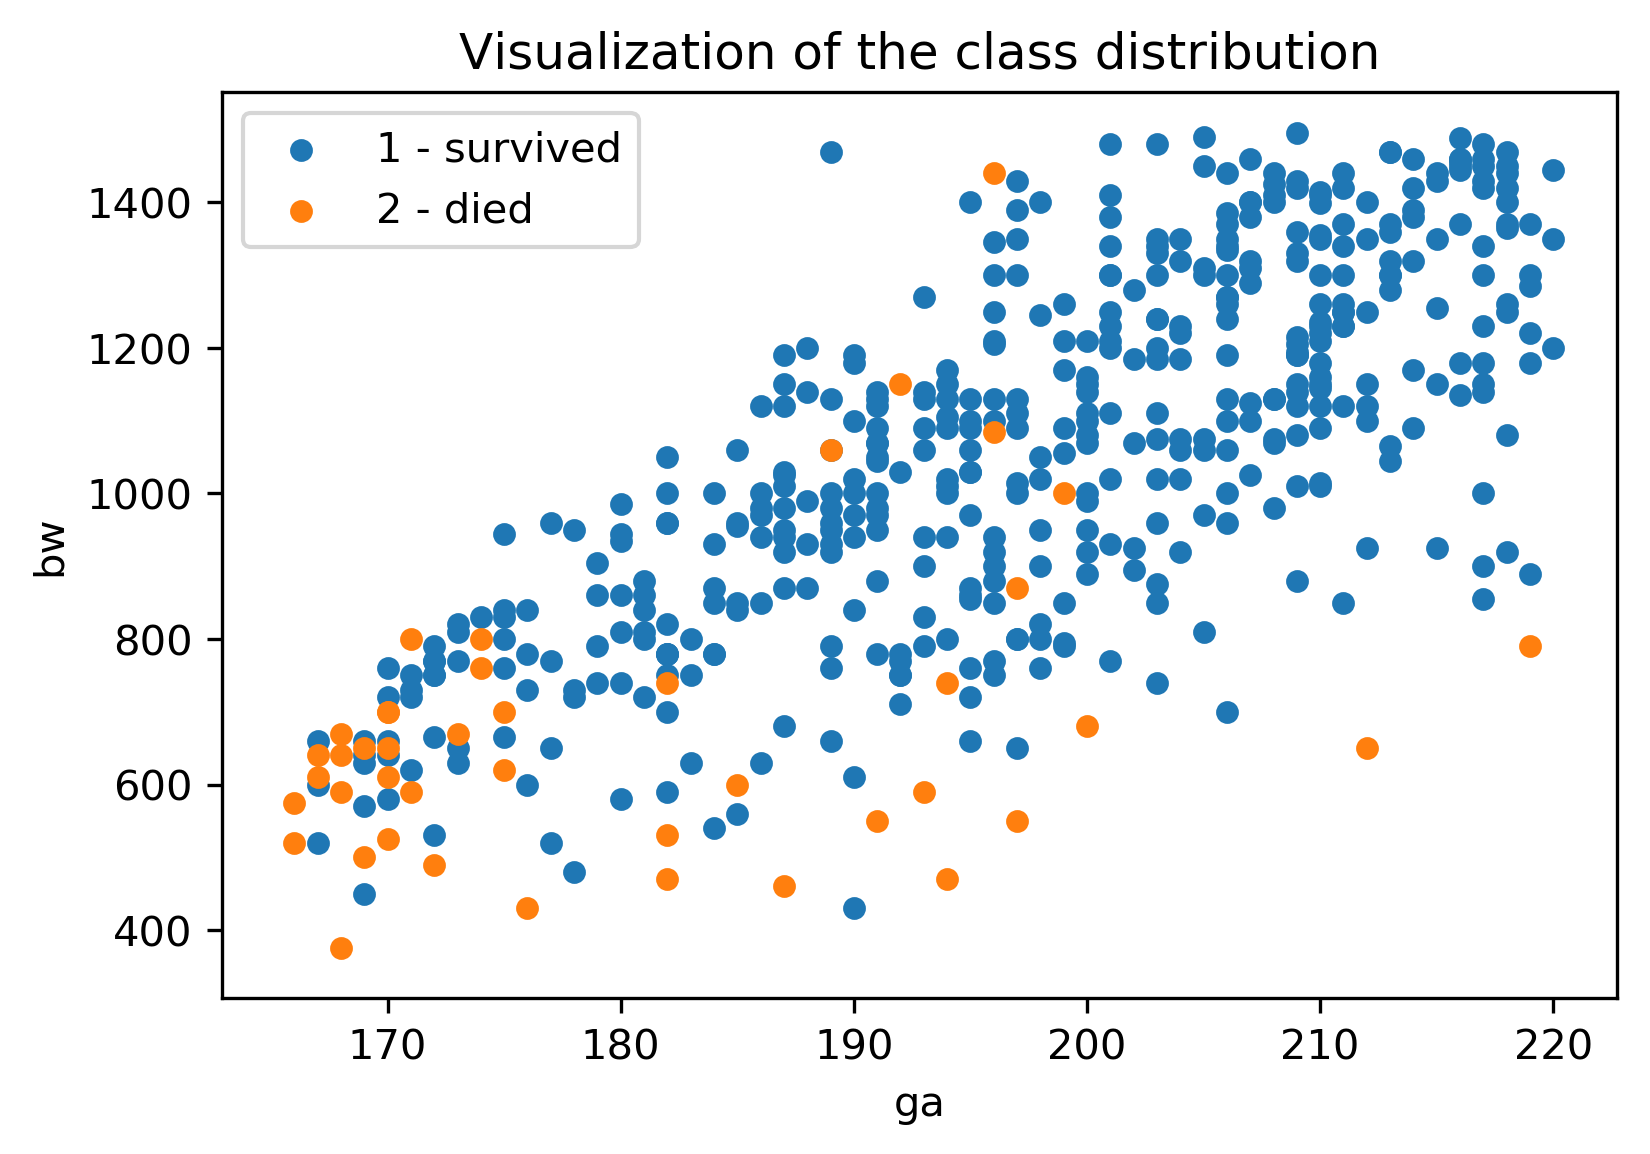
\includegraphics{raw_vis.png}
    \caption{Distribution of the training data}
    \label{fig:training}
\end{figure}

\section{Method}

In order to build a strong machine learning algorithm that can predict accurately the in-hospital mortality we used and evaluated a wide range of existing ML methods, that are used for binary classification. The ML methods we used are:

\begin{itemize}
    \item Logistic Regression
    \item Decision Trees
    \item Support Vector Machine (SVM)
    \item Gaussian Naive Bayes
    \item Gaussian Processes
\end{itemize}

Those methods were then applied separately to the basic data set and to the extracted statistics from the time-series data and eventually to the combined information of both data sets.

The following subsections give a short explanation of the different methods used.

\subsection*{Logistic Regression}

Logistic regression is a regression model where the dependent variable is categorical. In our case the dependent variable is a binary variable. But logistic regression can also be applied to cases where the dependent variable has more than two outcome categories, it is then called multinomial logistic regression.

Logistic regression uses a  predictor map $ h(.)$ with $h ( \mathbf { x } ) \in [ 0,1] $. One common choice for the predictor function $h$ is the so-called sigmoid function $ \sigma ( z ) $:
$$ h ^ { ( \mathbf { w } ,b ) } ( \mathbf { x } ) = \sigma \left( \mathbf { w } ^ { T } \mathbf { x } + b \right) \text{ with } \sigma ( z ) : = \frac{1}{1+ \exp ( - z )}  $$

In contrast to linear regression there is no closed form solution for the cost-minimising parameters, which is why gradient descent is used to find those optimal parameters.

\subsection*{Decision Trees}

Decision trees are very a very useful tool when predicting a target value as a trained decision tree is simple to understand and to interpret. Classification trees are a type of tree models where the target variable is a discrete set of values. In these tree structures, the leaves represent those class labels and branches represent conjunctions of features that lead to those class labels.

When constructing or learning the tree structure the algorithm generally work top-down and choose those conjunctions of features at each step that best splits the set of items. Depending on the algorithm different metrics are used to choose the 'best' conjunction of features. But generally these metrics measure the homogeneity of the target variable within the subsets.

\subsection*{Support Vector Machine}

Support Vector Machines (SVM) construct a hyperplane in a high- dimensional space, which then is  used for classification or regression. The premise of SVM is to select a particular hyperplane which results in a  good separation of training points. A good separation is achieved by a hyperplane that has the largest distance to the nearest training-data point of any class. In other words SVM finds those hyperplane that maximise the  functional margin. After the training a SVM are used to categorise the test data according to on which side of the hyperplane the prediction lies.

\subsection*{Gaussian Naive Bayes}

In general naive Bayes classifiers are the Bayesian adaptation of a probabilistic classifiers, they apply Bayes' theorem with strong (\textit{naive}) independence assumptions between the features.
For continuous data one typically assumes a gaussian distribution of the data within each class.

First the data has to be segmented by the class, then the mean and variance in each class has to be computed. $ \mu _{k}$ is the mean of the values in $x$ and  $ \sigma _{k}^{2}$ denotes the variance of the values in $x$ associated with class $C_k$.
The probability of some observation value $v$ given a class $C_{k}$ follows then Normal distribution parameterised by $\mu _{k}$ and $\sigma _{k}^{2}$:
$$  p(x=v\mid C_{k})={\frac {1}{\sqrt {2\pi \sigma _{k}^{2}}}}\,e^{-{\frac {(v-\mu _{k})^{2}}{2\sigma _{k}^{2}}}} $$

%\subsection*{Gaussian Processes}

\subsection{Modelling of basic data}
In the case of the basic data, we can build classifiers on the base of the two collected features gestational age at birth $ga$ and birth weight $bw$. Therefore, we applied and assessed the above reported classification methods. For assessing each individual classifier, we verified some of the most common score that can be computed during the training, namely mis-classification count, precision, recall, and accuracy. However, we spent time also checking visually that the classifier produced meaningful results. This visual check can be done by plotting the classification results on the test set and verify that graphically they resemble the training set. The objective is to select sensible classifier for this particular task. After checking both the scores and the results on the test set, the selected classifiers become part of a voting system. In this voting system it is sufficient that only one classifier labels a data point as "died", to have "died" as final classification for that data point. From a medical prospective, this is a safe choice, since it reduces the possibility of false negative.

\subsection{Modelling time-series data}
In order to model time-series data, we decided to extract the following statistics from each time-series:
\begin{itemize}
    \item Mean and variance
    \item Intercept and slope of linear regression on the data
\end{itemize}

On the base of this feature extrapolation, we applied the same classifiers presented above. Again, by checking both visually and the scores obtained by the different classifiers, one can select sensible classifiers to be part of the final voting system. In this case to graphically check the results on the test set, we mapped back the results on time-series in the $(ga, bw)$ space of the basic data.

\subsection{Combining both data frames}

Ultimately we augment the basic data with the information gained from the time-series data mentioned in the section above. This should theoretically lead to a richer data set and we hope to build better classifiers by combining the information of both the basic and the time-series data.

\section{Results}
In this section, the results on basic data (\ref{sec:res_basic_data}), time-series data (\ref{sec:res_ts_data}) and the combination of the two data sets (\ref{sec:res_comb_data}) are presented.

\subsection{Basic data}\label{sec:res_basic_data}
The score of the tested method on the training set are reported in Table~\ref{tab:basicdatascores}. Average mis-classification count, precision, recall and accuracy over the results of 5-fold cross validation on the training set are reported. In addition, in Figure~\ref{fig:basicdatatest} the results on the test set for the different classifier are presented.

\begin{table}[H]
    \centering
    \begin{tabular}{|c|c|c|c|c|}
    \hline
        Classifier & mis-classification count & Precision & Recall & Accuracy \\
    \hline
        Gaussian Processes (RBF)& 8.0   & 0.986 & 0.919 & 0.929\\
        SVM (RBF)               & 14.0  & 0.866 & 0.859 & 0.977\\
        Decision tree           & 12.19 & 0.943 & 0.877 & 0.924\\
        Logistic regression     & 8.0   & 0.995 & 0.919 & 0.923\\
        Gaussian Naive Bayes    & 10.6  & 0.925 & 0.893 & 0.956\\
    \hline
    \end{tabular}
    \caption{Average mis-classification count, precision, recall and accuracy over the results of 5-fold cross validation on the training set.}
    \label{tab:basicdatascores}
\end{table}

\begin{figure}[H]
    \centering
    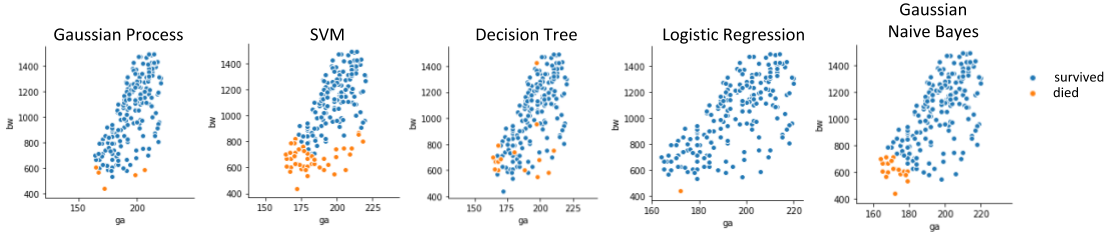
\includegraphics[width=\linewidth]{basicdata.png}
    \caption{\textbf{Basic data}: Classifier results on the test set.}
    \label{fig:basicdatatest}
\end{figure}

By combining the predictions of the different classifiers, we obtain the results reported in Figure~\ref{fig:basicdatacomb}. In this case, it is sufficient for a data point to be classified as "died" by only one classifier to be classified as "died" in these results. This is a conservative approach as we want to build a classifier, which reduces the false positives in its predictions.

\begin{figure}[H]
    \centering
    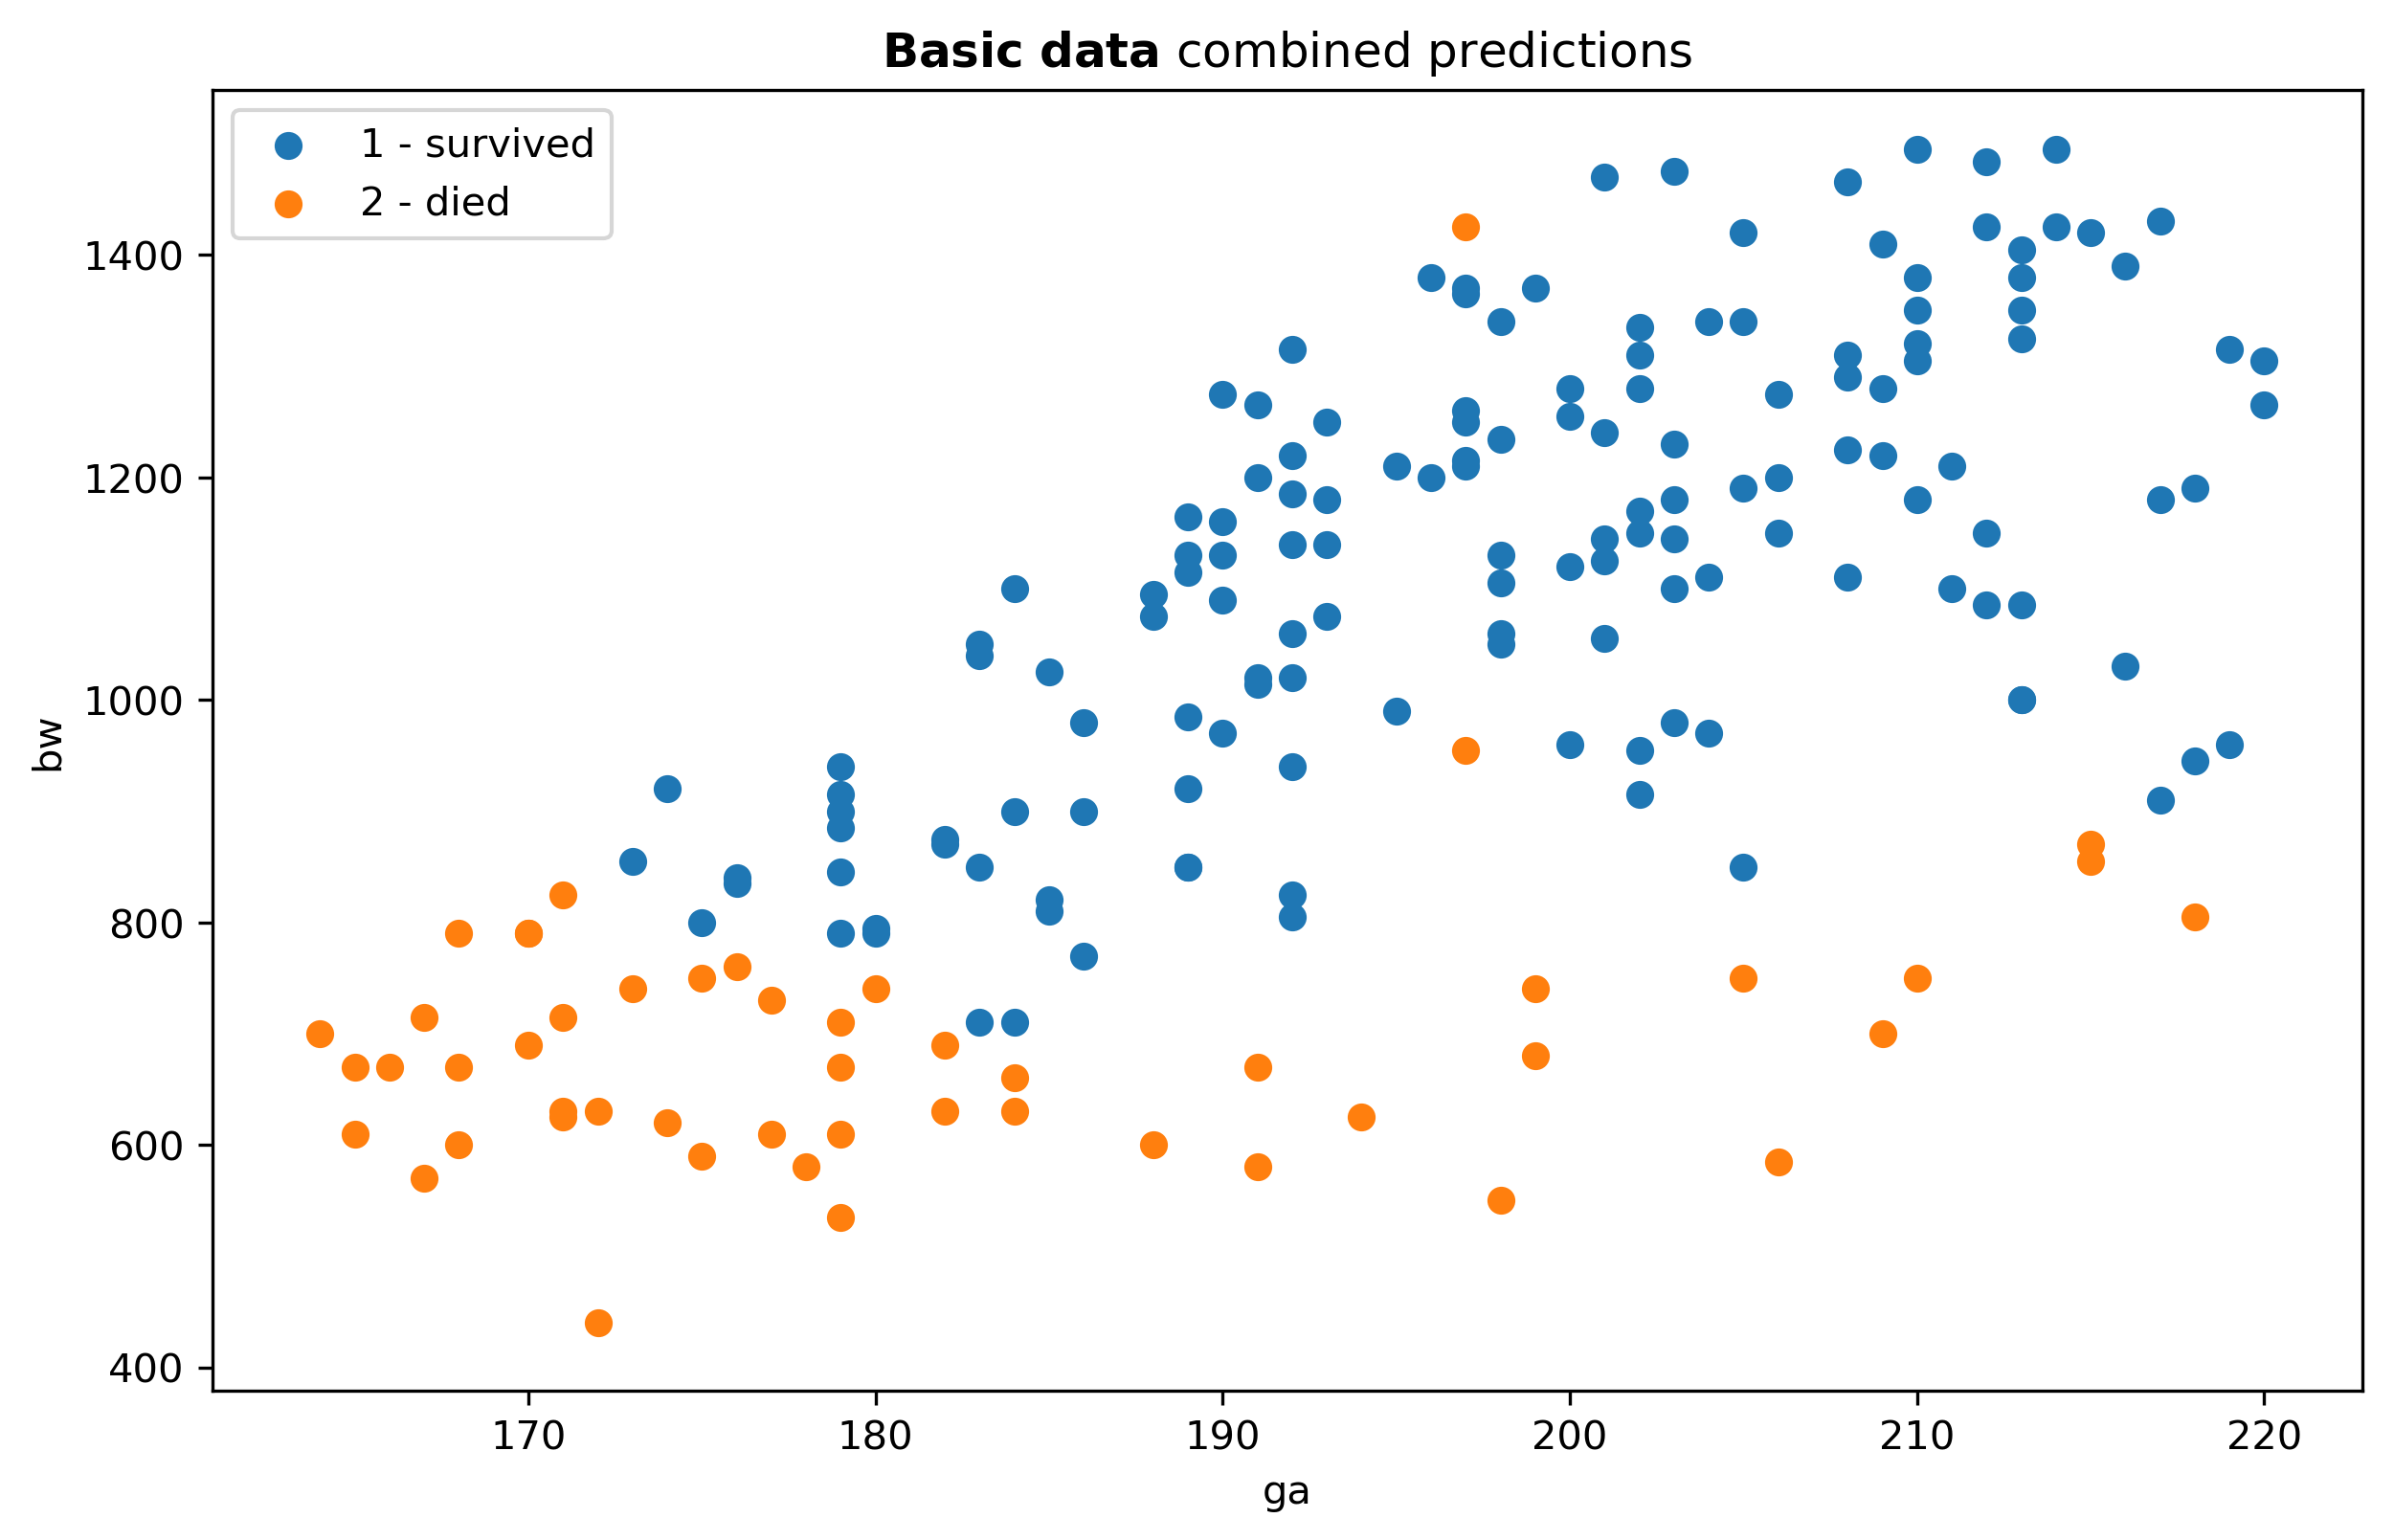
\includegraphics[width=0.7\linewidth]{basic_data_combined.png}
    \caption{Classification results obtained by combining the opinions of different classifiers on the test set}
    \label{fig:basicdatacomb}
\end{figure}

\subsection{Time-series data}\label{sec:res_ts_data}
As for the basic data, the score of the tested method on the training set are reported in Table~\ref{tab:tsscores}. Average mis-classification count, precision, recall and accuracy over the results of 5-fold cross validation on the training set are reported. In addition, in Figure~\ref{fig:tstest} the results on the test set for the different classifier are presented. It is important to notice that the results of the classification has been plotted in the feature space of the basic data in order to get a meaningful visualization. Regarding Figure~\ref{fig:combtest} we did not include the Gaussian Naive Bayes classifier as it provides a very aggressive classification.

\begin{table}[H]
    \centering
    \begin{tabular}{|c|c|c|c|c|}
    \hline
        Classifier & mis-classification count & Precision & Recall & Accuracy \\
    \hline
        Gaussian Processes (RBF)& 9.0   & 0.986 & 0.909 & 0.920\\
        SVM (RBF)               & 28.0  & 0.727 & 0.719 & 0.959\\
        Decision tree           & 15.80 & 0.881 & 0.841 & 0.942\\
        Logistic regression     & 8.59  & 0.995 & 0.914 & 0.917\\
        Gaussian Naive Bayes    & 45.39 & 0.526 & 0.546 & 0.962\\
    \hline
    \end{tabular}
    \caption{Average mis-classification count, precision, recall and accuracy over the results of 5-fold cross validation on the training set.}
    \label{tab:tsscores}
\end{table}

\begin{figure}[H]
    \centering
    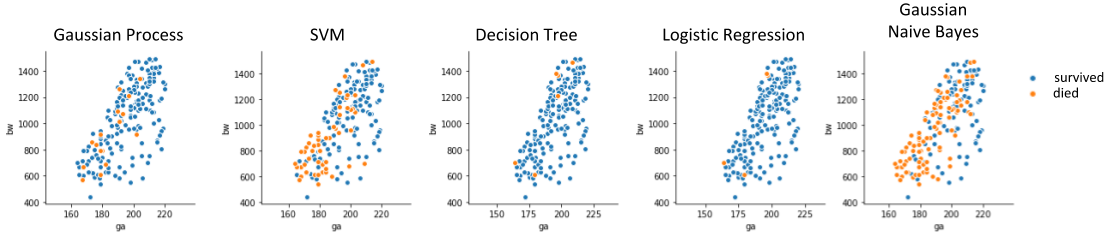
\includegraphics[width=\linewidth]{ts.png}
    \caption{\textbf{Time-series data}: Classifier results on the test set.}
    \label{fig:tstest}
\end{figure}

By combining the predictions of the different classifiers, we obtain the results reported in Figure~\ref{fig:tscomb}. As for the basic data, it is sufficient for a data point to be classified as "died" by only one classifier to be classified as "died" in these results.

\begin{figure}[H]
    \centering
    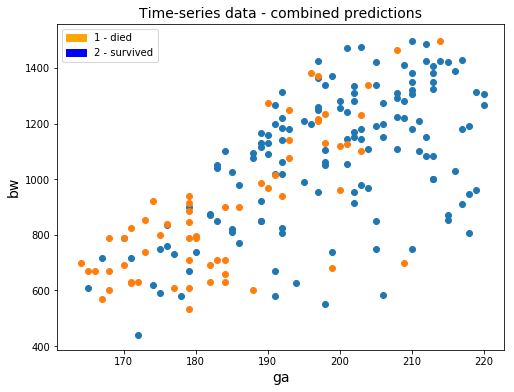
\includegraphics[width=0.7\linewidth]{ts_combined.png}
    \caption{Classification results obtained by combining the opinions of different classifiers on the test set}
    \label{fig:tscomb}
\end{figure}

\subsection{Basic data and time-series data combined}\label{sec:res_comb_data}
As for the basic and time-series data, the score of the tested method on the training set are reported in Table~\ref{tab:combscores}. Average mis-classification count, precision, recall and accuracy over the results of 5-fold cross validation on the training set are reported. In addition, in Figure~\ref{fig:combtest} the results on the test set for the different classifier are presented. It is important to notice that the results of the classification has been plotted in the feature space of the basic data in order to get a meaningful visualization. Regarding Figure~\ref{fig:combtest} we did not include the Gaussian Naive Bayes classifier as it provides a very aggressive classification.

\begin{table}[H]
    \centering
    \begin{tabular}{|c|c|c|c|c|}
    \hline
        Classifier & mis-classification count & Precision & Recall & Accuracy \\
    \hline
        Gaussian Processes (RBF)& 8.59  & 0.986 & 0.914 & 0.924\\
        SVM (RBF)               & 17.6  & 0.831 & 0.823 & 0.972\\
        Decision tree           & 10.6  & 0.942 & 0.893 & 0.941\\
        Logistic regression     & 9.19  & 0.980 & 0.908 & 0.923\\
        Gaussian Naive Bayes    & 33.79 & 0.650 & 0.662 & 0.970\\
    \hline
    \end{tabular}
    \caption{Average mis-classification count, precision, recall and accuracy over the results of 5-fold cross validation on the training set.}
    \label{tab:combscores}
\end{table}

\begin{figure}[H]
    \centering
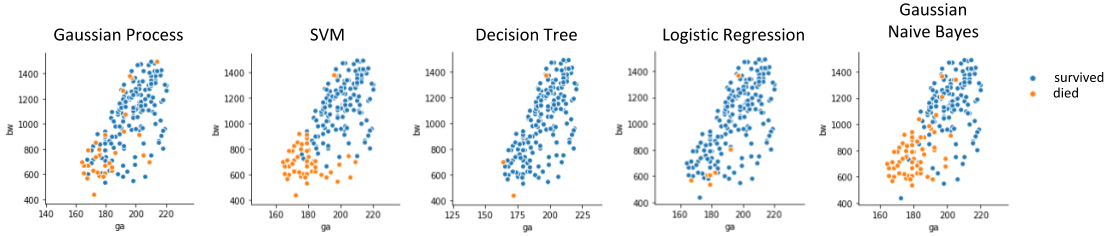
\includegraphics[width=\linewidth]{combined_data.png}
    \caption{\textbf{Combined data}: Classifier results on the test set.}
    \label{fig:combtest}
\end{figure}

By combining the predictions of the different classifiers, we obtain the results reported in Figure~\ref{fig:comb}. As for the basic and time-series data, it is sufficient for a data point to be classified as "died" by only one classifier to be classified as "died" in these results.

\begin{figure}[H]
    \centering
    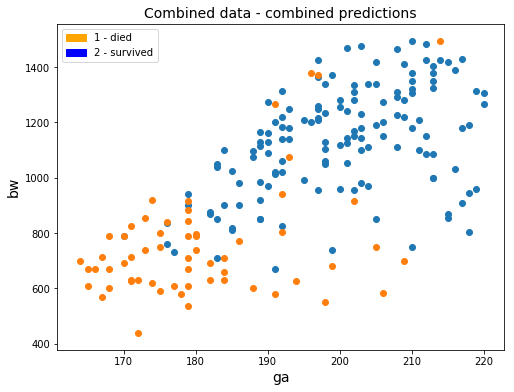
\includegraphics[width=0.7\linewidth]{combined.png}
    \caption{Classification results obtained by combining the opinions of different classifiers on the test set}
    \label{fig:comb}
\end{figure}

As a results, the following list summarises the patient ID's in the test set that have been classified as not surviving the NICU: 501, 502, 520, 522, 532, 533, 536, 540, 541, 542, 543, 547, 548, 549, 551, 552, 563, 564, 566, 567, 574, 587, 590, 591, 592, 597, 599, 604, 606, 607, 608, 609, 611, 613, 614, 615, 625, 627, 635, 639, 640, 644, 648, 649, 652, 654, 659, 663, 665, 666, 669, 680, 682, 685, 686, 688, 691, 693, 696, 697


\section{Discussion}\label{sec:discussion}
In this section we discuss the results obtained on the basic data, the time-series data and finally the combined data.

\subsection*{Basic data}\label{sec:dis_basic_data}
% basic data good for prediction
What we can see from the results in Table~\ref{tab:basicdatascores} is that on average the methods that are performing less in terms of mis-classification count (SVM, decision tree and Gaussian naive Bayes), are the ones that actually are learning more from the data. This can be clearly seen from the plots of the results on the test set reported in Figure~\ref{fig:basicdatatest}. Moreover, by combining the classification from the different methods, we can clearly see that the separation that is learned is the area under more or less 800g. With this split of the data we can actually produce meaningful prediction.

\subsection*{Time-series data}\label{sec:dis_ts_data}
% ts data not good for prediction
As we can see from the results on time-series, the pattern is not so clear as in the basic data. In particular, the Gaussian Naive Bayes classifier is producing very confusing data. Therefore, our sensible choice has been to ignore it in the combination of the classification results. However, it seems that time-series data are not contributing significantly to improve the performance of the model.


\subsection*{Basic data and time-series data combined}\label{sec:dis_comb_data}
% comb data a bit better  for prediction than basic
In conclusion, by combining the two data set, we can clearly see that the classifiers are relying more on the basic data. This can be noticed by looking at the predictions on the test set. Again, Gaussian Naive Bayes predictions are quite confusing. Hence, we excluded this classifier from the final combined prediction. We believe that the combined results reported in Figure~\ref{fig:comb} can be considered our final classification results. They represent the combination of the good baseline provided by the basic data and the information added through time-series data.


\section{Conclusion}

The task of this report was to predict in-hospital mortality based on simulated data.
We used various classifiers ranging from logistic regression and decision trees to SVMs and Gaussian naive Bayes and finally Gaussian processes to make a robust binary classification.
Those classifiers were applied to the basic data set and the time-series data set alone and eventually to the combined data set. In order to gain one global prediction we merged the separate classifiers with the rule, that it is sufficient for a data point to be classified as "died" if only one classifier labels the data point as "died".

As discussed in chapter \ref{sec:discussion} we can conclude that the basic data set alone is already giving a reasonably good amount of information for predicting in-hospital mortality. On the contrary the time-series data set does not contain enough information in order to build a robust classifier. Hence a pure reliance on the time-series data is not recommended and information covered in the basic data should be rather used.

When both data sets are combined the predictions are strongly influenced by the basic data set. Which is why we suggest to focus on gaining more information in the same style as the basic data set rather than time-series data. Other single-valued patient scores like Apgar, CRIB-II, SNAP-II or SNAPPE-II should be added for a more precise prediction of the in-hospital mortality. Values contained in those scores are generally easy to compute by hand and do not need special equipment. Examples of additional values are: skin color, pulse rate, activity, respiration effort, sex, admission temperature. There are many more values one could add to enrich the basic data and which help the mentioned classifies to give more accurate and robust predictions. 

%\section{References}
%\addcontentsline{toc}{section}{References}
%\bibliographystyle{unsrt}
%\bibliography{bib}

\section{Appendix}
The following pages show our source code for building the classifiers. 


\end{document}